% =====================================================================
%  CENG 252 -- Practice Midterm 2: Solutions
% =====================================================================
\documentclass[11pt]{article}
\usepackage[margin=2.2cm,headheight=14pt]{geometry}
\usepackage{amsmath,amssymb}
\usepackage[version=4]{mhchem}
\usepackage{tikz}
\usepackage{pgfplots}
\pgfplotsset{compat=1.17}
\usepackage[most]{tcolorbox}
\usepackage{booktabs,array,tabularx}
\usepackage{enumitem}
\usepackage{fancyhdr}
\usepackage{lmodern}
\usepackage[T1]{fontenc}

\setlength{\parindent}{0pt}
\setlength{\parskip}{4pt}
\pagestyle{fancy}
\fancyhf{}
\lhead{\small CENG 252 \textbullet\ Practice Midterm 2 \textbullet\ Solutions}
\rhead{\small Lectures 1--10}
\cfoot{\small \thepage}

\definecolor{keyblue}{RGB}{0,84,147}
\definecolor{warnred}{RGB}{176,30,30}
\definecolor{tipgreen}{RGB}{20,110,60}
\newtcolorbox{answer}{enhanced,breakable,colback=keyblue!5,colframe=keyblue,title={Answer},fonttitle=\bfseries,left=4pt,right=4pt,top=2pt,bottom=2pt}
\newtcolorbox{mistake}[1][Common mistake]{enhanced,breakable,colback=warnred!5,colframe=warnred,title={#1},fonttitle=\bfseries,left=4pt,right=4pt,top=2pt,bottom=2pt}
\newtcolorbox{grading}{enhanced,breakable,colback=tipgreen!5,colframe=tipgreen,title={Grading guide},fonttitle=\bfseries,left=4pt,right=4pt,top=2pt,bottom=2pt}
\newtcolorbox{keyidea}[1][Key idea]{enhanced,breakable,colback=black!3,colframe=black!60,title={#1},fonttitle=\bfseries,left=4pt,right=4pt,top=2pt,bottom=2pt}

\newcommand{\AS}[1]{\mathrm{#1\!\cdot\!S}}
\newcommand{\step}[1]{\par\smallskip\textbf{Step #1.}\ }

\begin{document}

\begin{center}
{\LARGE\bfseries CENG 252 Practice Midterm 2: Solutions}\\[4pt]
Lectures 1--10 \quad\textbullet\quad 100 points \quad\textbullet\quad 80 minutes
\end{center}

\begin{center}
\small
\renewcommand{\arraystretch}{1.35}
\begin{tabularx}{\textwidth}{c X l}
\toprule
Problem & Final answers & Similar to (Fogler 5th ed.)\\
\midrule
1 & $\Delta H^\circ_{Rx}=-6000$ cal/mol, $\Delta C_P=0$; $T=300+120X$; at $X=0.6$: $T=372$ K, $k=0.652$ min$^{-1}$,
$K_C=4.28$, $X_e=0.81$, $V=177$ dm$^3$; $X=0.8$ impossible ($X_e(396\text{ K})=0.72$) & Ex.~11-2, 11-3(c), 11-4\\
2 & $I_0/I=1+\dfrac{k_3}{k_2C_M+k_4}C_Q$; $k'=0.50$ L/mmol, $C_Q=6.0$ mmol/L; $V_{\max}=2.0$ mmol/(L$\cdot$min),
$K_M=4.0$ mmol/L; $t=27.2$ min & Ex.~9-1, 9-2, 9-3\\
3 & $-r_C'=\dfrac{k(P_C-P_BP_P/K_P)}{1+K_CP_C+K_BP_B}$; initial rates: linear, levelling off, constant; surface reaction
limiting, $k=0.50$ mol/(kg$\cdot$s$\cdot$atm), $K_C=1.0$ atm$^{-1}$; $W=30$ kg (20 kg if benzene is ignored) & \S10.3, Ex.~10-2(b)\\
4 & $r''_{\text{Dep}}=\dfrac{k'P_{\mathrm{GeCl_2}}P_{\mathrm{H_2}}}{\left(1+K_AP_{\mathrm{GeCl_2}}+\sqrt{K_HP_{\mathrm{H_2}}}\right)^3}$;
in GeCl$_4$: $\propto\dfrac{P_{\mathrm{GeCl_4}}P_{\mathrm{H_2}}P_{\mathrm{Cl_2}}^2}{(\ldots)^3}$; $P^*=0.25$ atm; orders $+1$ and $-2$ & \S10.5.2\\
\bottomrule
\end{tabularx}
\end{center}

\begin{keyidea}[How this exam maps to the instructor's announcement]
\begin{itemize}[itemsep=1pt]
\item ``One problem on energy balance (non-isothermal steady state)'' $\to$ \textbf{Problem 1}. It is pitched at
Ex.~11-2 (heat of reaction), Ex.~11-3(c) (adiabatic CSTR at the exit $T$) and the \emph{strategy} of Ex.~11-4. As
promised, it does not ask you to solve for the adiabatic equilibrium $T$ and $X$.
\item ``Chapter 9 (9.1--9.3), Ex.~9-1, 9-2, 9-3'' $\to$ \textbf{Problem 2}: a Stern--Volmer derivation, $V_{\max}$ and $K_M$ from data, and a batch enzymatic reactor.
\item ``10.3 (benzene decomposition) is very important'' $\to$ \textbf{Problem 3}, plus the hand-calculation part of
Ex.~10-2 (fluidised CSTR). No $X$ or $P$ profiles are integrated, as promised.
\item ``10.5.2 (CVD) is very important'' $\to$ \textbf{Problem 4}.
\end{itemize}
Timing: a well-prepared student needs about 18 + 13 + 20 + 14 = 65 minutes, which leaves about 15 minutes to check.
\end{keyidea}

% =====================================================================
\section*{Problem 1: Energy balance, adiabatic CSTR (25 pts)}

\subsection*{(a) Heat of reaction}
\[
\Delta H^\circ_{Rx}=H_B^\circ-H_A^\circ=-41{,}000-(-35{,}000)=-6000\ \text{cal/mol A}\quad(\text{exothermic}),
\]
\[
\Delta C_P=C_{P,B}-C_{P,A}=40-40=0 .
\]
\begin{answer}
$\Delta H^\circ_{Rx}=-6000$ cal/mol A. Since $\Delta C_P=0$, $\Delta H_{Rx}(T)=\Delta H^\circ_{Rx}(T_R)+\Delta C_P(T-T_R)=-6000$
cal/mol at every temperature.
\end{answer}

\subsection*{(b) Adiabatic $T$--$X$ relation}
\step{1}Adiabatic ($\dot Q=0$), no shaft work ($\dot W_s=0$), all species fed at $T_0$, and $\Delta C_P=0$:
\[
-F_{A0}\sum\Theta_iC_{P,i}(T-T_0)-\Delta H^\circ_{Rx}F_{A0}X=0
\quad\Rightarrow\quad
T=T_0+\frac{(-\Delta H^\circ_{Rx})X}{\sum\Theta_iC_{P,i}} .
\]
\step{2}$\Theta_B=0$ and $\Theta_I=0.20/0.80=0.25$, so
$\sum\Theta_iC_{P,i}=C_{P,A}+\Theta_IC_{P,I}=40+0.25(40)=50$ cal/(mol A$\cdot$K).
\begin{answer}
\[
T=300+\frac{6000}{50}X=300+120X\ \text{(K)}
\]
\end{answer}
\begin{mistake}
Leaving out the inert ($\sum\Theta_iC_{P,i}=40$ gives $T=300+150X$, which is too hot). $\Theta_I$ is per mole of \emph{A} fed:
$0.20/0.80$, not 0.20.
\end{mistake}

\subsection*{(c) CSTR volume for $X=0.60$}
A CSTR operates entirely at its exit conditions, so evaluate everything at $X=0.60$.

\step{1}Exit temperature: $T=300+120(0.60)=372$ K. \quad $\dfrac{1}{300}-\dfrac{1}{372}=6.452\times10^{-4}$ K$^{-1}$.

\step{2}Rate constant:
$k=0.005\exp\!\left[\dfrac{15{,}000}{1.987}(6.452\times10^{-4})\right]=0.005\,e^{4.870}=0.652$ min$^{-1}$.

\step{3}Equilibrium constant (exothermic, so $K_C$ falls):
$K_C=30\exp\!\left[\dfrac{-6000}{1.987}(6.452\times10^{-4})\right]=30\,e^{-1.948}=4.28$.

\step{4}Feasibility check: $X_e=\dfrac{K_C}{1+K_C}=\dfrac{4.28}{5.28}=0.81>0.60$. \checkmark

\step{5}Liquid-phase stoichiometry: $C_A=C_{A0}(1-X)=0.80$ and $C_B=C_{A0}X=1.20$ mol/dm$^3$:
\[
-r_A=k\left(C_A-\frac{C_B}{K_C}\right)=0.652\left(0.80-\frac{1.20}{4.28}\right)=0.652(0.520)=0.339\ \text{mol/(dm}^3\cdot\text{min)}.
\]
\step{6}$F_{A0}=0.80(125)=100$ mol/min:
\[
V=\frac{F_{A0}X}{-r_A}=\frac{(100)(0.60)}{0.339}.
\]
\begin{answer}
$V\approx$ \textbf{177 dm$^3$} (with $v_0=F_{A0}/C_{A0}=50$ dm$^3$/min, $\tau=3.5$ min), operating at 372 K.
For comparison, an \emph{isothermal} CSTR at 300 K would need about 15{,}800 dm$^3$. The heat released by the
reaction speeds it up roughly 90-fold.
\end{answer}
\begin{mistake}
(1) Using $k$ and $K_C$ at the \emph{feed} temperature. (2) Using the $X_e$ of the adiabatic equilibrium point instead of $X_e$
at the reactor temperature. (3) Writing $-r_A=kC_A$ and dropping the reverse term.
\end{mistake}

\subsection*{(d) The adiabatic limit}
(i) At $X=0.80$ the energy balance gives $T=300+120(0.80)=396$ K. There,
\[
K_C=30\exp\!\left[\frac{-6000}{1.987}\left(\frac{1}{300}-\frac{1}{396}\right)\right]=30\,e^{-2.440}=2.61,\qquad X_e=\frac{2.61}{3.61}=0.72 .
\]
\begin{answer}
(i) To reach $X=0.80$, the adiabatic feed must heat up to 396 K. At that temperature equilibrium allows only
$X_e=0.72<0.80$, so \textbf{no adiabatic reactor of any size can reach 0.80}. (For reference, the adiabatic equilibrium point
is at about 390 K and $X\approx0.75$; you were not asked to find it.)

(ii) The equilibrium curve $X_e(T)$ falls with $T$ (exothermic). The energy-balance line rises from $(T_0,0)$ with slope
$\sum\Theta_iC_{P,i}/(-\Delta H^\circ_{Rx})$. They intersect at the adiabatic equilibrium point. Ways to go higher:
\begin{itemize}[itemsep=1pt]
\item a \textbf{lower feed temperature} $T_0$ (the line shifts left; $T_0=280$ K gives about 0.80);
\item \textbf{more inert} (larger $\sum\Theta_iC_{P,i}$, so the line is steeper and $T$ rises less);
\item \textbf{reactors in series with interstage cooling}, or removing heat (a non-adiabatic reactor).
\end{itemize}
\end{answer}

\begin{center}
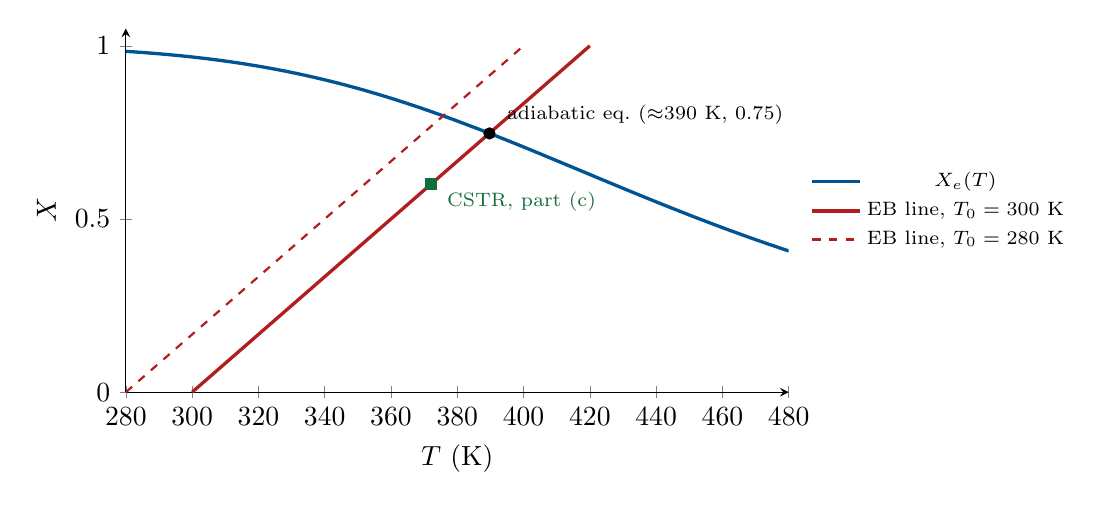
\begin{tikzpicture}
\begin{axis}[width=10cm,height=6.2cm,xmin=280,xmax=480,ymin=0,ymax=1.05,axis lines=left,
  xlabel={$T$ (K)},ylabel={$X$},legend style={font=\scriptsize,at={(1.02,0.5)},anchor=west,draw=none}]
\addplot[very thick,keyblue,domain=280:480,samples=120]{30*exp(-3019.6*(1/300-1/x))/(1+30*exp(-3019.6*(1/300-1/x)))};
\addlegendentry{$X_e(T)$}
\addplot[very thick,warnred,domain=300:420]{(x-300)/120};
\addlegendentry{EB line, $T_0=300$ K}
\addplot[thick,dashed,warnred,domain=280:400]{(x-280)/120};
\addlegendentry{EB line, $T_0=280$ K}
\addplot[only marks,mark=*,mark size=2pt] coordinates{(389.7,0.747)};
\node[font=\scriptsize,anchor=west] at (axis cs:392,0.80) {adiabatic eq.\ ($\approx$390 K, 0.75)};
\addplot[only marks,mark=square*,mark size=2pt,tipgreen] coordinates{(372,0.6)};
\node[font=\scriptsize,anchor=west,tipgreen] at (axis cs:374,0.55) {CSTR, part (c)};
\end{axis}
\end{tikzpicture}
\end{center}

\begin{grading}
(a) 2 for $\Delta H^\circ_{Rx}$ with its sign and basis, 1 for $\Delta C_P=0$ and the consequence.
(b) 2 for reducing the energy balance to the adiabatic form, 2 for $\Theta_I$ and $\sum\Theta_iC_{P,i}$, 2 for $T=300+120X$.
(c) 1 for $T$, 2 for $k$, 2 for $K_C$, 1 for the $X_e$ check, 2 for the rate with stoichiometry, 2 for $V$.
(d) 3 for (i) with the $X_e(396)$ calculation, 3 for (ii): sketch, intersection and two valid fixes.
\end{grading}

% =====================================================================
\section*{Problem 2: Reaction pathways and enzymes (20 pts)}

\subsection*{(a) Stern--Volmer equation}
\step{1}Write the rate of every step for D$^*$:
formation $=I_a$;\; loss by (2) $=k_2C_MC_{D^*}$;\; by (3) $=k_3C_QC_{D^*}$;\; by (4) $=k_4C_{D^*}$.

\step{2}PSSH on D$^*$:
\[
0=I_a-k_2C_MC_{D^*}-k_3C_QC_{D^*}-k_4C_{D^*}
\quad\Rightarrow\quad
C_{D^*}=\frac{I_a}{k_2C_M+k_3C_Q+k_4}.
\]
\step{3}Intensity with and without quencher:
\[
I=k_4C_{D^*}=\frac{k_4I_a}{k_2C_M+k_3C_Q+k_4},\qquad I_0=I(C_Q=0)=\frac{k_4I_a}{k_2C_M+k_4}.
\]

\step{4}Take the ratio:
\begin{answer}
\[
\frac{I_0}{I}=\frac{k_2C_M+k_3C_Q+k_4}{k_2C_M+k_4}=1+k'C_Q,\qquad k'=\frac{k_3}{k_2C_M+k_4}
\]
$C_M$ (the solvent) is constant, so the Stern--Volmer plot of $I_0/I$ against $C_Q$ is a straight line with intercept 1.
$I_a$ (and $k_4$) cancel because the same lamp excites the dye in both measurements: the ratio isolates the competition
for D$^*$.
\end{answer}

\subsection*{(b) Numbers}
\begin{answer}
$k'=\dfrac{2.5-1}{3.0}=$ \textbf{0.50 L/mmol}. For $I=I_0/4$: $I_0/I=4=1+0.50\,C_Q\Rightarrow C_Q=$ \textbf{6.0 mmol/L}.
\end{answer}

\subsection*{(c) Lineweaver--Burk}
\begin{center}
\renewcommand{\arraystretch}{1.25}
\begin{tabular}{lcccc}
\toprule
$1/C_S$ (L/mmol) & 1.000 & 0.500 & 0.250 & 0.125\\
$1/(-r_S)$ (L$\cdot$min/mmol) & 2.50 & 1.50 & 1.00 & 0.75\\
\bottomrule
\end{tabular}
\end{center}
Slope $=\dfrac{2.50-0.75}{1.000-0.125}=2.0$ min; \quad intercept $=2.50-2.0(1.000)=0.50$ L$\cdot$min/mmol.
\begin{answer}
$V_{\max}=1/0.50=$ \textbf{2.0 mmol/(L$\cdot$min)}; \quad $K_M=\text{slope}\times V_{\max}=2.0\times2.0=$ \textbf{4.0 mmol/L}.
\end{answer}

\subsection*{(d) Batch reactor at half the enzyme loading}
\step{1}$V_{\max}=k_{\text{cat}}C_{E,t}$ is proportional to the enzyme loading, so at 0.50 g/L, $V_{\max}=1.0$ mmol/(L$\cdot$min).
$K_M=(k_2+k_3)/k_1$ is a ratio of rate constants and does \textbf{not} depend on the amount of enzyme: $K_M=4.0$ mmol/L.

\step{2}Mole balance: $\dfrac{dC_S}{dt}=-\dfrac{V_{\max}C_S}{K_M+C_S}\;\Rightarrow\;-\displaystyle\int_{C_{S0}}^{C_S}\left(\frac{K_M}{C_S}+1\right)dC_S=V_{\max}t$, so
\[
t=\frac{K_M}{V_{\max}}\ln\frac{1}{1-X}+\frac{C_{S0}X}{V_{\max}}.
\]
\step{3}$t=\dfrac{4.0}{1.0}\ln10+\dfrac{(20)(0.90)}{1.0}=9.2+18.0$.
\begin{answer}
$t=$ \textbf{27.2 min}. Halving the enzyme loading halves $V_{\max}$ and doubles the time; $K_M$ is unchanged.
\end{answer}
\begin{mistake}
Scaling $K_M$ with the enzyme loading, or using the CSTR formula $t=C_{S0}X/(-r_S)$ for a batch reactor.
\end{mistake}

\begin{grading}
(a) 2 for the step rates, 2 for the PSSH and $C_{D^*}$, 2 for the ratio, 1 for why $I_a$ cancels.
(b) 1.5 + 1.5. (c) 2 for the reciprocals and fit, 2 for $V_{\max}$ and $K_M$ with units.
(d) 2 for the scaling argument, 2 for the integrated batch equation, 2 for 27.2 min.
\end{grading}

% =====================================================================
\section*{Problem 3: Cumene decomposition (30 pts)}

\subsection*{(a) Surface reaction limiting}
\step{1}RLS rate law. The forward step is single-site; the reverse is P from the gas attacking B$\cdot$S:
\[
-r_C'=r_S=k_S\left(C_{\AS{C}}-\frac{P_PC_{\AS{B}}}{K_S}\right).
\]
\step{2}The fast steps are at equilibrium:
\[
\frac{r_{AD}}{k_A}=P_CC_v-\frac{C_{\AS{C}}}{K_C}\approx0\Rightarrow C_{\AS{C}}=K_CP_CC_v;\qquad
\frac{r_D}{k_D}=C_{\AS{B}}-K_BP_BC_v\approx0\Rightarrow C_{\AS{B}}=K_BP_BC_v .
\]
\step{3}Substitute:
$r_S=k_SC_v\left(K_CP_C-\dfrac{K_BP_BP_P}{K_S}\right)=k_SK_CC_v\left(P_C-\dfrac{P_BP_P}{K_P}\right)$, using $K_P=\dfrac{K_CK_S}{K_B}$.

\step{4}Site balance (P is not adsorbed): $C_t=C_v+C_{\AS{C}}+C_{\AS{B}}=C_v(1+K_CP_C+K_BP_B)$.
\begin{answer}
\[
-r_C'=\frac{k\left(P_C-P_BP_P/K_P\right)}{1+K_CP_C+K_BP_B},\qquad k=k_SK_CC_t
\]
There is no $P_P$ term in the denominator, because propylene does not adsorb.
\end{answer}

\subsection*{(b) Initial rates}
Pure cumene feed: $P_B=P_P=0$ at the inlet.
\begin{answer}
\begin{itemize}[itemsep=1pt]
\item Adsorption-limited: $-r_{C0}'=k_AC_tP_{C0}$, \textbf{linear}, with no levelling off.
\item Surface-reaction-limited: $-r_{C0}'=\dfrac{kP_{C0}}{1+K_CP_{C0}}$, linear at low $P_{C0}$, then \textbf{levels off} at $k/K_C$.
\item Desorption-limited: with $P_P=0$ the denominator is just $K_SK_CP_{C0}$, so $-r_{C0}'=k_DC_t$, \textbf{independent of $P_{C0}$}.
With no propylene, B$\cdot$S cannot react back, the surface fills with B, and the rate is set by how fast B leaves.
\end{itemize}
\end{answer}
\begin{center}
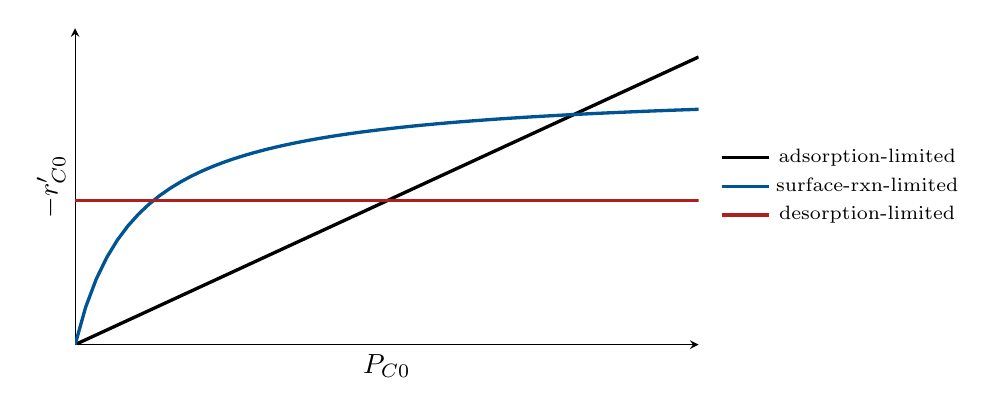
\begin{tikzpicture}
\begin{axis}[width=9.5cm,height=5.6cm,xmin=0,xmax=10,ymin=0,ymax=2.2,axis lines=left,ticks=none,
  xlabel={$P_{C0}$},ylabel={$-r_{C0}'$},legend style={font=\scriptsize,at={(1.02,0.5)},anchor=west,draw=none}]
\addplot[very thick,black,domain=0:10]{0.2*x};\addlegendentry{adsorption-limited}
\addplot[very thick,keyblue,domain=0:10,samples=60]{1.8*x/(1+x)};\addlegendentry{surface-rxn-limited}
\addplot[very thick,warnred,domain=0:10]{1.0};\addlegendentry{desorption-limited}
\end{axis}
\end{tikzpicture}
\end{center}
\begin{mistake}
Writing the desorption-limited initial rate as proportional to $P_{C0}$. You must set $P_P=0$ \emph{before} simplifying: the
$P_P$ terms vanish from the denominator, and $P_{C0}$ cancels.
\end{mistake}

\subsection*{(c) Identifying the RLS and its parameters}
The rate rises and levels off, so the \textbf{surface reaction is rate-limiting}, as Fogler found for the real cumene data.
Linearise: $\dfrac{P_{C0}}{-r_{C0}'}=\dfrac{1}{k}+\dfrac{K_C}{k}P_{C0}$.
\begin{center}
\renewcommand{\arraystretch}{1.25}
\begin{tabular}{lccccc}
\toprule
$P_{C0}$ (atm) & 0.5 & 1.0 & 2.0 & 4.0 & 8.0\\
$P_{C0}/(-r_{C0}')$ (atm$\cdot$kg$\cdot$s/mol) & 3.0 & 4.0 & 6.0 & 10.0 & 18.0\\
\bottomrule
\end{tabular}
\end{center}
Slope $=\dfrac{18.0-3.0}{8.0-0.5}=2.0$ kg$\cdot$s/mol; \quad intercept $=3.0-2.0(0.5)=2.0$ atm$\cdot$kg$\cdot$s/mol.
\begin{answer}
$k=1/2.0=$ \textbf{0.50 mol/(kg cat$\cdot$s$\cdot$atm)}; \quad $K_C=\text{slope}\times k=$ \textbf{1.0 atm$^{-1}$}.
\end{answer}
\begin{center}
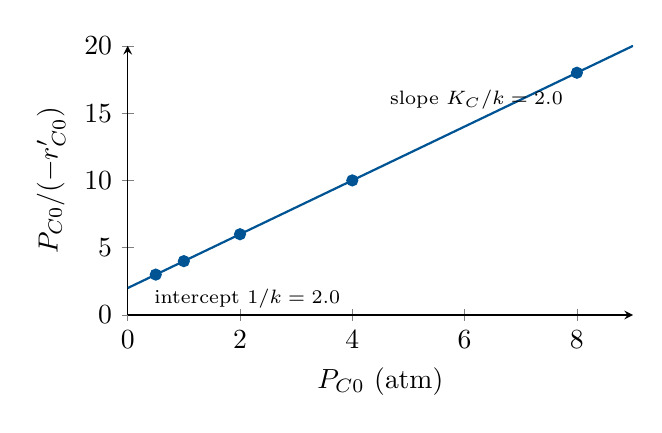
\begin{tikzpicture}
\begin{axis}[width=8cm,height=5cm,axis lines=left,xmin=0,xmax=9,ymin=0,ymax=20,
  xlabel={$P_{C0}$ (atm)},ylabel={$P_{C0}/(-r_{C0}')$}]
\addplot[only marks,mark=*,keyblue] coordinates{(0.5,3)(1,4)(2,6)(4,10)(8,18)};
\addplot[thick,keyblue,domain=0:9]{2+2*x};
\node[font=\scriptsize,anchor=west] at (axis cs:0.3,1.2) {intercept $1/k=2.0$};
\node[font=\scriptsize,anchor=west] at (axis cs:4.5,16) {slope $K_C/k=2.0$};
\end{axis}
\end{tikzpicture}
\end{center}

\subsection*{(d) Fluidised CSTR}
\step{1}Stoichiometry: pure C, \ce{C -> B + P}: $\delta=1$, $\varepsilon=1$. Isothermal, no $\Delta P$:
\[
P_C=P_0\frac{1-X}{1+X}=3\cdot\frac{0.5}{1.5}=1.0\ \text{atm},\qquad P_B=P_P=P_0\frac{X}{1+X}=1.0\ \text{atm}.
\]
\step{2}Exit rate (irreversible form):
$-r_C'=\dfrac{kP_C}{1+K_CP_C+K_BP_B}=\dfrac{0.5(1.0)}{1+1.0+1.0}=0.167$ mol/(kg$\cdot$s).

\step{3}$W=\dfrac{F_{C0}X}{-r_C'}=\dfrac{(10)(0.5)}{0.167}=30$ kg.
\begin{answer}
$W=$ \textbf{30 kg}. Ignoring benzene: $-r_C'=0.5/2=0.25$, so $W=20$ kg, an underestimate by a \textbf{factor of 1.5}.
Benzene, the product, occupies sites that cumene needs (product inhibition). The CSTR runs entirely at the exit composition,
where $P_B$ is high, so the effect is large.
\end{answer}
\begin{mistake}
Using $P_C=P_0(1-X)$ (that is, $\varepsilon=0$). One mole of gas becomes two, so the mole fraction of cumene is diluted
by the factor $1+X$.
\end{mistake}

\begin{grading}
(a) 2 for the RLS rate law with the reverse term, 3 for the equilibrium expressions, 2 for the site balance, 1 for the final form.
(b) 1 for each initial rate, 3 for the sketch.
(c) 2 for the identification with a reason, 3 for the linearisation and table, 3 for $k$ and $K_C$ with units.
(d) 3 for $\varepsilon$ and the partial pressures, 2 for the rate, 2 for $W$, 1 for the factor 1.5 with the reason.
\end{grading}

% =====================================================================
\section*{Problem 4: CVD of germanium (25 pts)}

\subsection*{(a) Deposition rate}
\step{1}RLS: $r''_{\text{Dep}}=k_Sf_{\mathrm{GeCl_2}}f_{\mathrm{H}}^2$.

\step{2}GeCl$_2$ adsorption at equilibrium:
\[
r_{AD}=k_A\left(f_vP_{\mathrm{GeCl_2}}-\frac{f_{\mathrm{GeCl_2}}}{K_A}\right)\approx0\;\Rightarrow\; f_{\mathrm{GeCl_2}}=K_AP_{\mathrm{GeCl_2}}f_v .
\]

\step{3}Dissociative H$_2$ adsorption at equilibrium (two sites in, two H atoms out):
\[
r_{AD,\mathrm{H_2}}=k_H\left(P_{\mathrm{H_2}}f_v^2-\frac{f_{\mathrm{H}}^2}{K_H}\right)\approx0\;\Rightarrow\; f_{\mathrm{H}}=\sqrt{K_HP_{\mathrm{H_2}}}\,f_v .
\]

\step{4}Substitute: $r''_{\text{Dep}}=k_SK_AK_HP_{\mathrm{GeCl_2}}P_{\mathrm{H_2}}f_v^3$.

\step{5}Area balance: $1=f_v+f_{\mathrm{GeCl_2}}+f_{\mathrm{H}}=f_v\left(1+K_AP_{\mathrm{GeCl_2}}+\sqrt{K_HP_{\mathrm{H_2}}}\right)$.
\begin{answer}
\[
r''_{\text{Dep}}=\frac{k'P_{\mathrm{GeCl_2}}P_{\mathrm{H_2}}}{\left(1+K_AP_{\mathrm{GeCl_2}}+\sqrt{K_HP_{\mathrm{H_2}}}\right)^3},\qquad k'=k_SK_AK_H
\]
(Fogler Eq.~10-90.)
\end{answer}

\subsection*{(b) In terms of GeCl$_4$}
The gas-phase equilibrium gives $K_P=\dfrac{P_{\mathrm{GeCl_2}}P_{\mathrm{Cl_2}}}{P_{\mathrm{GeCl_4}}}$, so
$P_{\mathrm{GeCl_2}}=\dfrac{K_PP_{\mathrm{GeCl_4}}}{P_{\mathrm{Cl_2}}}$. Substitute, then multiply the top and bottom by $P_{\mathrm{Cl_2}}^3$:
\begin{answer}
\[
r''_{\text{Dep}}=\frac{k'K_P\,P_{\mathrm{GeCl_4}}P_{\mathrm{H_2}}P_{\mathrm{Cl_2}}^2}{\left[P_{\mathrm{Cl_2}}\left(1+\sqrt{K_HP_{\mathrm{H_2}}}\right)+K_AK_PP_{\mathrm{GeCl_4}}\right]^3}
\]
If H$_2$ is weakly adsorbed this becomes $\dfrac{kP_{\mathrm{GeCl_4}}P_{\mathrm{H_2}}P_{\mathrm{Cl_2}}^2}{(P_{\mathrm{Cl_2}}+K_AK_PP_{\mathrm{GeCl_4}})^3}$
(Fogler Eq.~10-91).
\textbf{Effect of Cl$_2$:} by Le Chatelier, Cl$_2$ pushes the gas-phase equilibrium back towards GeCl$_4$, which lowers
$P_{\mathrm{GeCl_2}}$, the species that actually adsorbs and deposits. At low GeCl$_2$ coverage the rate goes as $1/P_{\mathrm{Cl_2}}$.
\end{answer}

\subsection*{(c) Optimum GeCl$_2$ pressure}
Let $a=1+\sqrt{K_HP_{\mathrm{H_2}}}=2.0$ and $P=P_{\mathrm{GeCl_2}}$, so $r''\propto\dfrac{P}{(a+K_AP)^3}$.
\[
\frac{d}{dP}\left[\frac{P}{(a+K_AP)^3}\right]=\frac{(a+K_AP)-3K_AP}{(a+K_AP)^4}=0
\;\Rightarrow\;
P^*=\frac{a}{2K_A}=\frac{2.0}{2(4.0)}.
\]
\begin{answer}
$P^*_{\mathrm{GeCl_2}}=$ \textbf{0.25 atm}. Apparent order in GeCl$_2$: \textbf{$+1$} at low pressure ($K_AP\ll a$), and
\textbf{$-2$} at high pressure ($r''\propto P/P^3$). Beyond $P^*$, GeCl$_2$ crowds out the H atoms it needs as reaction partners.
\end{answer}
\begin{center}
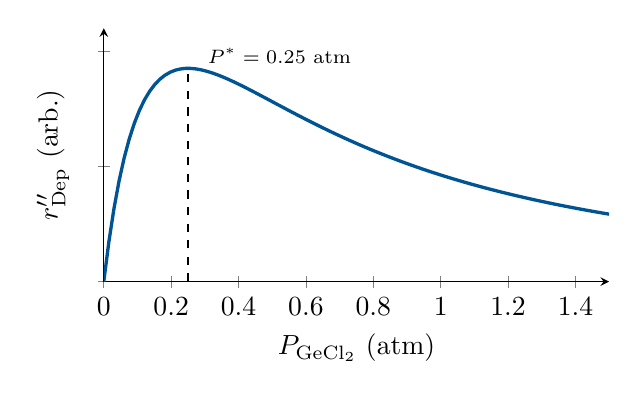
\begin{tikzpicture}
\begin{axis}[width=8cm,height=4.8cm,axis lines=left,xmin=0,xmax=1.5,ymin=0,ymax=0.011,
  xlabel={$P_{\mathrm{GeCl_2}}$ (atm)},ylabel={$r''_{\text{Dep}}$ (arb.)},yticklabels={},
  scaled y ticks=false]
\addplot[very thick,keyblue,domain=0:1.5,samples=100]{x/(2+4*x)^3};
\addplot[dashed] coordinates{(0.25,0)(0.25,0.00926)};
\node[font=\scriptsize,anchor=west] at (axis cs:0.28,0.0098) {$P^*=0.25$ atm};
\end{axis}
\end{tikzpicture}
\end{center}

\subsection*{(d) Concepts}
\begin{answer}
\begin{enumerate}[label=(\roman*),itemsep=1pt]
\item The RLS needs \textbf{three} sites at once (one GeCl$_2\cdot$S and two H$\cdot$S), so the rate contains $f_v^3$, and the
area balance turns that into a cubed denominator.
\item H$_2$ adsorbs \textbf{dissociatively} into two H atoms, so $f_{\mathrm{H}}^2\propto P_{\mathrm{H_2}}f_v^2$, giving $f_{\mathrm{H}}\propto\sqrt{P_{\mathrm{H_2}}}$.
\item Three occupied sites react, and two vacant sites are released, but the newly deposited Ge atom is \textbf{itself a new
surface site}: three sites before, three after. The area balance stays valid as the film grows.
\end{enumerate}
\end{answer}
\begin{mistake}
(1) $f_{\mathrm{H}}=K_HP_{\mathrm{H_2}}f_v$ (no square root). (2) A squared denominator (counting two sites instead of three).
(3) Writing the rate in terms of GeCl$_4$ directly: GeCl$_4$ never adsorbs, only GeCl$_2$ does.
\end{mistake}

\begin{grading}
(a) 2 for the RLS rate, 2 for $f_{\mathrm{GeCl_2}}$, 3 for $f_{\mathrm{H}}$ with the square root, 2 for the area balance, 1 for the final form.
(b) 3 for the substitution, 2 for the Cl$_2$ explanation.
(c) 3 for the derivative and $P^*$, 1 for the number, 2 for both orders.
(d) 1 + 1 + 2.
\end{grading}

\end{document}
